\documentclass[11pt,a4paper]{article}
\usepackage[margin=2.2cm]{geometry}
\usepackage{amsmath,amssymb,xcolor,enumitem,booktabs,graphicx}
\usepackage[normalem]{ulem}
\setlength{\parskip}{0.6em}\setlength{\parindent}{0pt}
\definecolor{newc}{HTML}{1f6f43}
\newcommand{\new}[1]{\textcolor{newc}{#1}}
\newcommand{\old}[1]{\textcolor{gray}{\sout{#1}}}
\newcommand{\note}[1]{{\small\itshape [#1]}}
\newcommand{\lab}[1]{\textsf{\footnotesize #1}}
\renewcommand{\ref}[1]{\lab{#1}}
\renewcommand{\eqref}[1]{(\lab{#1})}
\newcommand{\nref}[1]{the (\lab{#1})}
\newcommand{\citep}[1]{[\lab{#1}]}
\newcommand{\citet}[1]{\lab{#1}}
\title{Proposed change, ``How an agent chooses its move''}
\date{24 November 2026, version 3 (Figure 13 with both halves)}
\begin{document}\sloppy
\maketitle

\section*{How to read this}
This answers part B of \texttt{method\_model\_comments.md} for
\lab{sec:method:model} in \texttt{4.Implementation.tex}, with the answers
of 24 November:
\begin{itemize}[nosep]
  \item B1: messages have no block of their own, and that is the thesis's
    own choice. The reason is that the agent's vector already comes from
    message passing over the graph.
  \item B4: no memory, because of the training cost and because the network
    is not the focus. Memory goes to future work. Leaving it out may favour
    the controllers that see more, which goes to the threats to validity.
  \item B5: the scale of 50, both a sentence on it and a threat at 64 agents.
  \item B8: Figure~13 keeps both halves, redrawn in greys with the words of the text.
  \item The rest (B2, B3, B5 first points, B6, B7, B8 small) is fixed as
    the comments say.
\end{itemize}
No equation changes its meaning, no parameter changes, and the code is
untouched. Two symbols go: $\mathrm{AGG}$ becomes the mean it always was,
and $\bar\xi_w(t)$ becomes $\xi_j(t)$ of the agent standing on $w$. Black
text stays, \new{green} is new and \old{struck} text goes.
\note{Notes in brackets} say why. Nothing below is in the thesis yet.

\section*{Part 1. What was checked}
\begin{itemize}[nosep]
  \item \textbf{Message passing} (\texttt{models/gnn\_encoder.py}). $\phi_r$
    reads the pair (vertex, neighbour), a linear layer and ReLU, and the
    mean over the neighbours follows. So a neighbour's weight is learned
    from both vertices' features. A graph convolution would weigh it by the
    degrees alone. This is the reason Appendix~C already gives.
  \item \textbf{Messages.} The sender's final vector, averaged over the
    agents heard, joined to the readout. No layer of its own. The
    readout feeds the move score, which is learned.
  \item \textbf{CRAMP.} Not in \texttt{thesis-progress/papers/}. The
    description of its message block (graph filters weighted by distance,
    over an image network's output) is taken from Appendix~C.
  \item \textbf{The scale of 50} (\texttt{observation.py},
    \texttt{DISTANCE\_SCALE}). The longest trip through a shelf, dock to
    shelf to workstation, is about 32 steps at 8 agents, 41 at 16, 55 at 32
    and 75 at 64 (Appendix~D instance report, 50 warehouses each). The
    label is the distance to the current target, one leg of that trip, so
    at 16 agents it stays below 1. At 64 agents it can pass 1.
  \item \textbf{Vertex features} \eqref{eq:features} hold the scaled
    distance $\eta_i(v,t)/50$ already. Only the words leave it out.
  \item \textbf{The value} is named in the training subsection (``a value
    head $V_\theta$''), so Figure~13 can name it.
\end{itemize}

\section*{Part 2. The section as it would read}

Every learned controller chooses moves with the same network. It reads the
part of the warehouse the agent sees and gives each possible move a score.
The simplest case is a decentralised agent, which runs the network on its
own field of view, and this subsection describes that case.
Section~\ref{sec:method:controllers} then shows what changes when agents
choose together. Figure~\ref{fig:architecture} shows the model in plain words.

\textbf{Figure 13 caption.} \old{The model in plain words. Every agent runs
the same network, and clashing moves become waits before the warehouse
moves on.} \new{One agent's network, left, and every agent running its own
copy, right. The value is used only in training
(Section~\ref{sec:method:training}).} \note{Placed with \texttt{[htbp]} after
this paragraph, so it no longer sits under the assignment text.}

\begin{center}
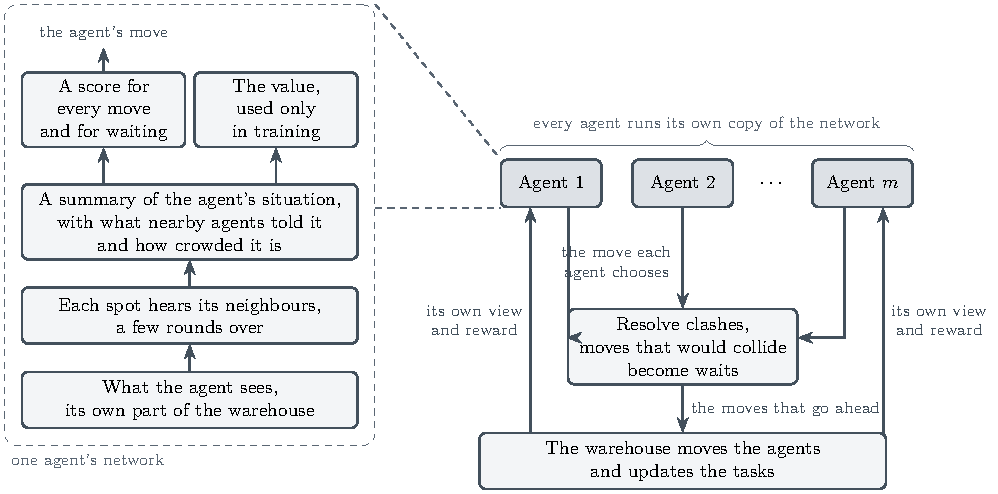
\includegraphics[width=\linewidth]{method_model_fig/architecture_proposed.pdf}
\end{center}
\note{Both halves stay (author, 24 November). The left shows what goes on
inside an agent. The right shows what Figure~12 does not: every agent runs
its own copy, on its own view, gets its own reward back, and the moves meet
only at resolving clashes. Redrawn in greys, with the words of the text
(``Resolve clashes'', ``the warehouse moves the agents and updates the
tasks''). Appendix~C keeps the compact figure, the same network with symbols
in van Knippenberg's form, next to the source comparison.}

The network follows \citet{vanKnippenberg2021}, who built on PRIMAL
\citep{sartoretti2019primal}. It keeps their local view and their distance
label\old{,}\new{. It} replaces their graph convolution \citep{kipf2017gcn}
with general message passing \citep{gilmer2017mpnn}\new{, so that a vertex
can weigh a neighbour by what is on it, such as an agent}. \old{and adds}
\new{It adds} messages between agents as in
\citet{pham2024optimizingcrowdawaremultiagentpath}.
Appendix~\ref{app:controllers:sources} sets the three side by side and
draws the model in the form of their figure.

\textbf{What the network reads.} Each vertex in view starts with a few
facts about itself. These are its role, how many steps nearer to or further
from the agent's target it is than the agent's own vertex, \new{how far it
is from the target,} whether an agent stands on it, and whether an earlier
agent in the same decision has chosen it. Together they are the
\emph{vertex features} $f(v,t)$~\eqref{eq:features}. The crowding feature
$\delta_i(t)$ is added once for the agent, not for each vertex. The
vertices chosen by earlier agents, including the vertex of an earlier agent
that chose to wait, form the set $\mathcal{V}_{\prec i}(t)$. It is always
empty for a decentralised agent, so every controller reads the same list
of features.

\textbf{Distance as a difference.} The target is often far away, so the
distance to it is a large number on every vertex in view. An agent 48 steps
from its target sees 48 where it stands and 47 one step closer. Only the
difference matters for the move. So each vertex gets its distance minus the
agent's own. This gives 0 where the agent stands, $-1$ one step closer and
$+1$ one step further. The number is then small like the other facts, and
the way to go is easy to read. It is capped at $\pm d_{\mathrm{obs}}$, so it
has the same range under every controller\new{, also when the window is the
whole warehouse}. \new{Formally, the \emph{relative distance label} is}
\begin{equation*}
  \tilde\eta_i(v,t) = \min\bigl(d_{\mathrm{obs}},\, \max\bigl(-d_{\mathrm{obs}},\,
    \eta_i(v,t) - \eta_i(\ell_i(t),t)\bigr)\bigr) .
  \tag{\lab{eq:relativeeta}}
\end{equation*}
\note{The display moves up from ``How far the target is'', where it did not
belong.}

\new{Figure~\ref{fig:distancedifference} shows the two numbers on a small
field of view.} \textbf{New figure, caption:} \new{The distance to the target
on each vertex in view, and the same minus the agent's own. Only the second
tells the way at a glance.}

\begin{center}
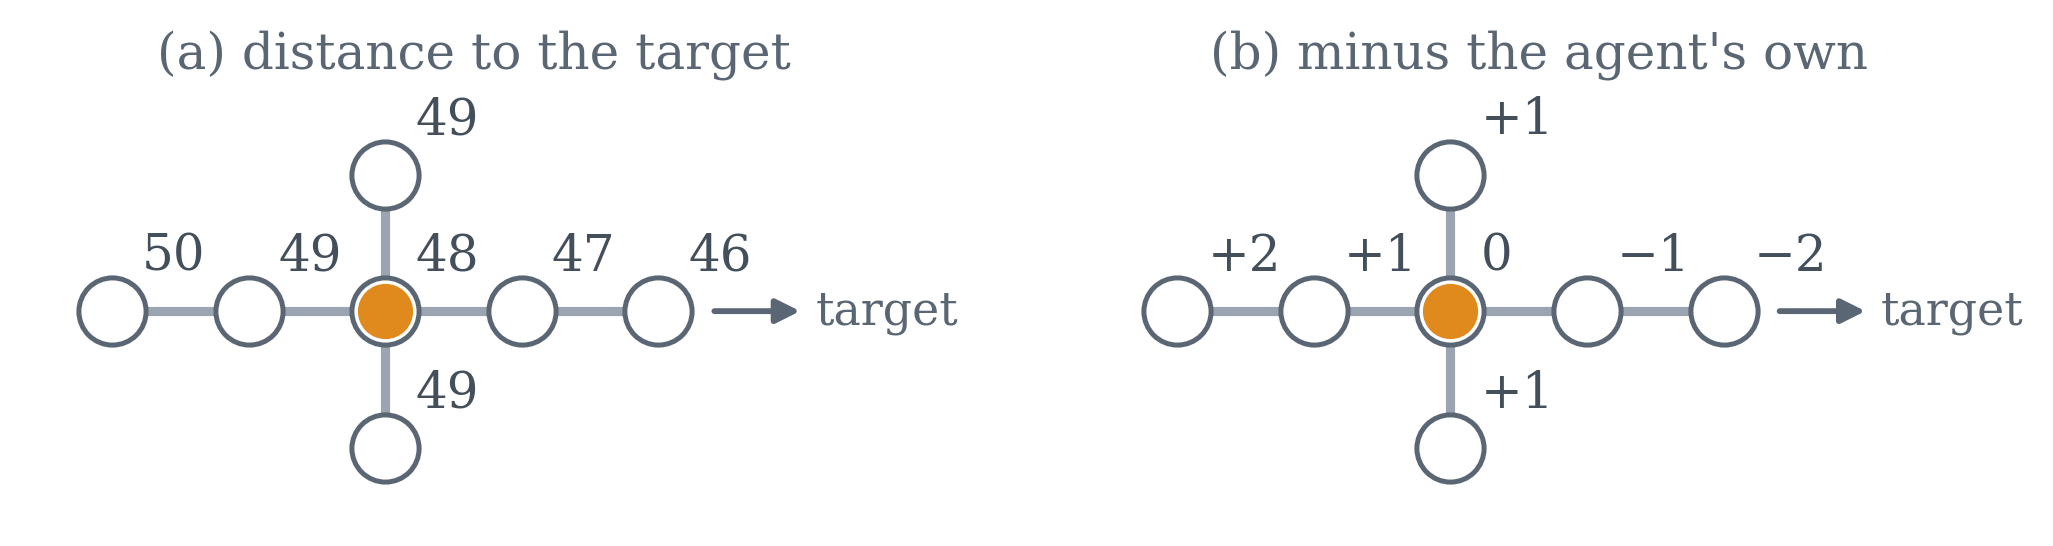
\includegraphics[width=0.85\linewidth]{method_model_fig/distance_difference.png}
\end{center}
\note{Script \texttt{scripts/images/distance\_difference.py}, viewer style:
aisle positions as white circles, the agent orange on its way to a pick.}

\textbf{How far the target is.} The difference shows the way but not how
far the target is, so an agent two steps from it would look the same as one
forty steps away. Each vertex therefore also gets its distance to the
target, as in \citet{vanKnippenberg2021}\old{, divided by $50$ so that it
stays near the range of the other facts. The same number is used in every
warehouse.}\new{. They give the raw distance. Here it is divided by $50$, the
\emph{scaled distance label} $\eta_i(v,t)/50$, so that it stays near the
range of the other facts. The 50 is the thesis's own round number, the same
in every warehouse, so the label means the same in each. In the 16-agent
warehouse the longest trip through a shelf is about 48 steps
(Appendix~\ref{app:instances:results}), so the label stays below 1 there.}
\note{The 50 was chosen on 4 November ([A82]), when the runs had 8 agents and
trips of about 30 steps. It is not a mistake and was not tuned. ``As in van
Knippenberg'' only covers the distance, not the division.} \old{Formally, the \emph{relative distance label} is [display]
and the \emph{scaled distance label} is $\eta_i(v,t)/50$.} The reward does
not use the label. It uses the distance left in the whole task, which also
counts the trip on from where the agent picks up \new{\eqref{eq:taskpotential}}.

\textbf{Passing information along the graph.} The network turns the field
of view into one vector $z_i$ for the agent in $L$ rounds. In each round
every vertex \new{hears its neighbours and} updates its own vector from
\old{those of its neighbours} \new{what it heard}, so after $L$ rounds a
vertex knows about the vertices up to $L$ \old{hops} \new{steps} away. The
agent's vector $z_i$ then joins three things. These are the final vector of
its own vertex, the mean of the messages \new{the agent} receives \new{from
other agents}, and the crowding feature. Formally, with
$h_v^{(0)} = f(v,t)$\new{, write $m_v^{(r)}$ for what vertex $v$ hears in
round $r$. Then}
\begin{align*}
  m_v^{(r)} &= \phi_r\bigl(h_v^{(r-1)},\, \{h_w^{(r-1)} : w \in
               \mathcal{G}_i^{(d_{\mathrm{obs}})}(t),\, (w,v)\in E \text{ or } (v,w)\in E\}\bigr),
  \tag{\lab{eq:msgpass}} \\
  h_v^{(r)} &= \psi_r\bigl(h_v^{(r-1)},\, m_v^{(r)}\bigr), \qquad r = 1,\dots,L,
  \\
  \xi_j(t) &= h_{\ell_j(t)}^{(L)},
  \tag{\lab{eq:message}} \\
  z_i &= h_{\ell_i(t)}^{(L)} \;\Vert\; \old{\mathrm{AGG}}\new{\mathrm{mean}}\bigl(\{\xi_j(t) :
        (a_i,a_j)\in E^{\mathcal{A}}_t\}\bigr) \;\Vert\; \delta_i(t) ,
  \tag{\lab{eq:readout}}
\end{align*}
where $\xi_j(t)$ is the message of agent $a_j$ \old{and $\mathrm{AGG}$ is
the mean}\new{, and $\Vert$ joins vectors end to end}. With $L=0$ each vertex
keeps its raw features. The number of rounds and the widths are set in
Appendix~\ref{app:training}.

\textbf{Messages.} \old{A message is the sender's own final vector, sent as
it is. No separate message layer is added, because a linear layer in front
of a mean and of the next linear layer adds no power.}
\new{A message has no layer of its own, and this is the thesis's own
choice. In \citet{pham2024optimizingcrowdawaremultiagentpath} an agent's
state comes from an image network over its grid window, so a separate
network is needed to pass it between agents. Here the agent's vector already
comes from message passing over the warehouse graph. A message is then one
more round of the same kind, along the communication
graph~\eqref{eq:commgraph}, with the mean collecting what arrives and the
move score after it doing the learning.} The weights are shared, so the
receiver's loss reaches the sender's vector and messages are trained
through the policy loss, as in
\citet{pham2024optimizingcrowdawaremultiagentpath} and \citet{li2022pico}.
Messages travel \old{one hop} \new{as far as the field of view} per
timestep, in one round only. More rounds would relay what agents beyond the
field of view send, and so widen the decentralised window past
$d_{\mathrm{obs}}$. A message is computed and used in the same timestep, so
the forward pass takes all agents of a timestep together. Execution stays
decentralised, since each agent still uses only its own view and the
messages it receives. With communication switched off, the message term is
dropped from \old{\nref{eq:readout}}\new{\eqref{eq:readout}}.
\note{``One hop'' meant one edge of the communication graph, which joins
agents up to $d_{\mathrm{obs}}$ apart, so ``as far as the field of view''
says it in the reader's terms.}

\textbf{Scoring each move by where it leads.} On a grid, ``north'' means
the same everywhere, which is what lets
\citet{pham2024optimizingcrowdawaremultiagentpath} use a fixed set of four
directions. On a graph a move has no name of its own. The only thing that
says what a move does is the vertex it leads to. So one small network,
shared by every edge, scores each move from the agent's vector $z_i$, the
vector of the vertex $w$ it leads to, and the message
\old{$\bar\xi_w(t)$} of the agent standing on $w$ if there is one. The wait
is scored from $z_i$ alone. Formally, \new{with $a_j$ the agent on $w$ and
$\xi_j(t)=0$ when $w$ is empty,} the \emph{move score} is
\begin{equation*}
  \mathrm{logit}(\mathrm{move\ to\ } w) = \mathrm{SCORE}_\theta\bigl(z_i \,\Vert\,
    h_w^{(L)} \,\Vert\, \old{\bar\xi_w(t)}\new{\xi_j(t)}\bigr), \qquad
  \mathrm{logit}(\mathrm{wait}) = \mathrm{SCORE}^{\mathrm{wait}}_\theta(z_i).
  \tag{\lab{eq:edgescore}}
\end{equation*}
Each move is thus judged by whether $w$ is closer to the target, whether it
is occupied, and, with communication on, what the agent standing there
reported. One score per candidate followed by a softmax is the pointer
mechanism of \citet{vinyals2015pointer}. The \old{head} \new{score} works
for any number of outgoing edges, and the numbering of the edges does not
affect what the policy learns. With communication switched off, the message
is dropped as well. Figure~\ref{fig:edgescore} shows the \new{scores} for
one agent.

\textbf{Figure 14 caption.} \old{The per-edge policy head of
\nref{eq:edgescore} for one agent. The same network scores every outgoing
edge, so the numbering of edges does not matter.} \new{The move scores of
agent $a_1$, on its way to a pick. Agent $a_2$, on its way to deliver, stands
on $w_2$, so that move's score also reads $a_2$'s message.} \note{Agents
coloured by what they do, as in the viewer.}

\begin{center}
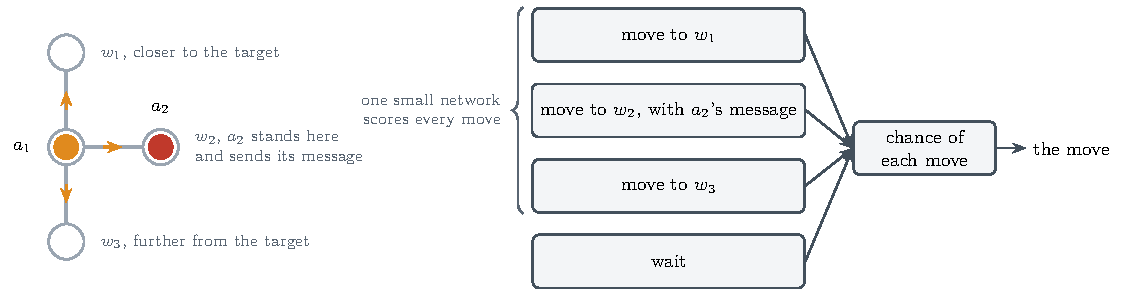
\includegraphics[width=\linewidth]{method_model_fig/edgescore_proposed.pdf}
\end{center}

\textbf{Only moves that exist.} The scores fill a fixed set of slots, one
for waiting and one for each outgoing edge in increasing vertex number, as
in \citet{vanKnippenberg2021}. \new{The slots only hold the scores in a fixed
order. Each score comes from the same network and the vertex the move leads
to, so the order of the slots does not change what the policy learns.} With
$d_{\max} = \max_{v\in V} |N^{+}(v)|$ there are $d_{\max}+1$ slots. At a
vertex with fewer edges, the empty slots get $-\infty$ before the softmax,
by the \emph{action mask}~\eqref{eq:mask}. So an agent can never choose a
move that does not exist. \citet{vanKnippenberg2021} instead turn such a
move into a penalised wait, and their policy has to learn not to choose it.

\textbf{No memory.} The network decides from what it sees now and does not
remember earlier steps. \old{Memory would be the same in every controller,
so it would not change the comparison, and it makes training much heavier.
PRIMAL gives its agents a memory network (an LSTM)
\citep{sartoretti2019primal}.} \new{PRIMAL \citep{sartoretti2019primal} and
\citet{pham2024optimizingcrowdawaremultiagentpath} both give their agents a
memory. The thesis takes the messages of the second but not its memory,
because memory makes training much heavier and the network is not what the
thesis studies.} \note{The fairness reason goes. Its doubt moves to the
Discussion, Part~3.}

\section*{Part 3. Discussion and future work}

\textbf{Threats to validity} (\texttt{5.Experiments.tex}, the list), two
new items:
\begin{itemize}[nosep]
  \item \new{No controller remembers earlier steps. The decentralised agent
    sees least, so it loses most from this, since an agent that leaves its
    view is forgotten. Leaving memory out may therefore favour the
    controllers that see more.}
  \item \new{The distance label is divided by one fixed number, 50. In the
    64-agent warehouse a trip reaches about 86 steps, so the label can pass 1
    and is no longer near the range of the other facts the network reads.}
\end{itemize}

\textbf{Future work} (\texttt{6.Conclusion.tex}, ``Future work''), one
line: \new{Giving the agents a memory, such as the LSTM of PRIMAL and CRAMP,
would show how much of the decentralised controller's gap comes from
forgetting what it saw.}

\section*{Part 4. Elsewhere}
\begin{itemize}[nosep]
  \item Notation tables (\texttt{2.Notation.tex}, \texttt{A.Notation.tex}):
    the row \old{$\bar\xi_w(t)$, vertex message} goes. The row for
    $\mathrm{SCORE}_\theta$ says ``\old{Per-edge policy head scoring}
    \new{One small network that scores} each move from the vertex it leads
    to, and the wait score''.
  \item The old \texttt{scripts/images/architecture.tex} and
    \texttt{edgescore.tex} are replaced by the two proposed files in
    \texttt{method\_model\_fig/}, then copied to \texttt{thesis/Images/}.
  \item \texttt{Appendix C} keeps its compact figure and its source
    comparison and its compact figure, whole. Its right half shows where
    the loop differs from van Knippenberg's, conflict resolution as a step
    of its own.
  \item \texttt{Appendix D}, \lab{app:instances:results}: the trip sentence
    gives 8 and 64 agents only. \new{At 16 agents the trips run from about
    13 to 41 steps.} is added, so the Method can point to it (instance
    report, 50 warehouses).
  \item New figure \lab{fig:distancedifference}, copied to
    \texttt{thesis/Images/}.
\end{itemize}

\section*{Questions}
None left. Approved on 24 November apart from Figure~13, which is now
redrawn with both halves.

\end{document}
